\documentclass{standalone}
\usepackage[T1]{fontenc}\usepackage{tikz}
\usepackage{amsmath, amsfonts}
\usetikzlibrary{arrows.meta}
\begin{document}
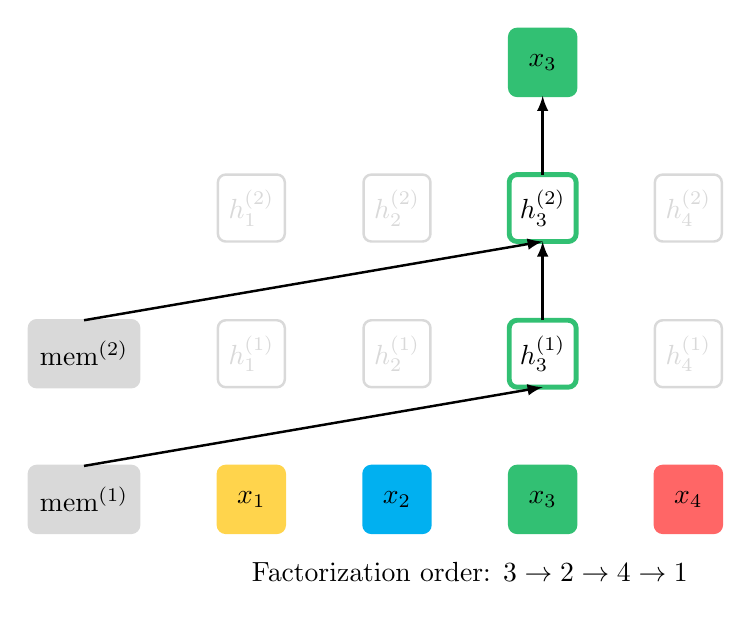
\begin{tikzpicture}
\definecolor{my_yellow}{RGB}{255,212,76}
\definecolor{my_green}{RGB}{50,192,115}
\definecolor{my_red}{RGB}{255,102,102}
\definecolor{my_blue}{RGB}{1,176,240}
\definecolor{my_grey}{RGB}{217,217,217}
\draw[rounded corners=0.100000cm, line width=0.031250cm, fill=my_grey, draw=my_grey] (-8.800000, -3.700000) -- (-7.400000, -3.700000) -- (-7.400000, -4.550000) -- (-8.800000, -4.550000) -- cycle;
\node[] at (-8.100000,-4.125000) {$\text{mem}^{(1)}$};
\draw[rounded corners=0.100000cm, line width=0.031250cm, fill=my_yellow, draw=my_yellow] (-6.400000, -3.700000) -- (-5.550000, -3.700000) -- (-5.550000, -4.550000) -- (-6.400000, -4.550000) -- cycle;
\node[] at (-5.975000,-4.125000) {$x_1$};
\draw[rounded corners=0.100000cm, line width=0.031250cm, fill=my_blue, draw=my_blue] (-4.550000, -3.700000) -- (-3.700000, -3.700000) -- (-3.700000, -4.550000) -- (-4.550000, -4.550000) -- cycle;
\node[] at (-4.125000,-4.125000) {$x_2$};
\draw[rounded corners=0.100000cm, line width=0.031250cm, fill=my_green, draw=my_green] (-2.700000, -3.700000) -- (-1.850000, -3.700000) -- (-1.850000, -4.550000) -- (-2.700000, -4.550000) -- cycle;
\node[] at (-2.275000,-4.125000) {$x_3$};
\draw[rounded corners=0.100000cm, line width=0.031250cm, fill=my_red, draw=my_red] (-0.850000, -3.700000) -- (0.000000, -3.700000) -- (0.000000, -4.550000) -- (-0.850000, -4.550000) -- cycle;
\node[] at (-0.425000,-4.125000) {$x_4$};
\draw[rounded corners=0.100000cm, line width=0.031250cm, fill=my_grey, draw=my_grey] (-8.800000, -1.850000) -- (-7.400000, -1.850000) -- (-7.400000, -2.700000) -- (-8.800000, -2.700000) -- cycle;
\node[] at (-8.100000,-2.275000) {$\text{mem}^{(2)}$};
\draw[rounded corners=0.100000cm, line width=0.031250cm, draw=my_grey] (-6.400000, -1.850000) -- (-5.550000, -1.850000) -- (-5.550000, -2.700000) -- (-6.400000, -2.700000) -- cycle;
\node[text=my_grey] at (-5.975000,-2.275000) {$h_1^{(1)}$};
\draw[rounded corners=0.100000cm, line width=0.031250cm, draw=my_grey] (-4.550000, -1.850000) -- (-3.700000, -1.850000) -- (-3.700000, -2.700000) -- (-4.550000, -2.700000) -- cycle;
\node[text=my_grey] at (-4.125000,-2.275000) {$h_2^{(1)}$};
\draw[rounded corners=0.100000cm, line width=0.031250cm, line width=0.062500cm, draw=my_green] (-2.700000, -1.850000) -- (-1.850000, -1.850000) -- (-1.850000, -2.700000) -- (-2.700000, -2.700000) -- cycle;
\node[] at (-2.275000,-2.275000) {$h_3^{(1)}$};
\draw[rounded corners=0.100000cm, line width=0.031250cm, draw=my_grey] (-0.850000, -1.850000) -- (0.000000, -1.850000) -- (0.000000, -2.700000) -- (-0.850000, -2.700000) -- cycle;
\node[text=my_grey] at (-0.425000,-2.275000) {$h_4^{(1)}$};
\draw[rounded corners=0.100000cm, line width=0.031250cm, draw=my_grey] (-6.400000, 0.000000) -- (-5.550000, 0.000000) -- (-5.550000, -0.850000) -- (-6.400000, -0.850000) -- cycle;
\node[text=my_grey] at (-5.975000,-0.425000) {$h_1^{(2)}$};
\draw[rounded corners=0.100000cm, line width=0.031250cm, draw=my_grey] (-4.550000, 0.000000) -- (-3.700000, 0.000000) -- (-3.700000, -0.850000) -- (-4.550000, -0.850000) -- cycle;
\node[text=my_grey] at (-4.125000,-0.425000) {$h_2^{(2)}$};
\draw[rounded corners=0.100000cm, line width=0.031250cm, line width=0.062500cm, draw=my_green] (-2.700000, 0.000000) -- (-1.850000, 0.000000) -- (-1.850000, -0.850000) -- (-2.700000, -0.850000) -- cycle;
\node[] at (-2.275000,-0.425000) {$h_3^{(2)}$};
\draw[rounded corners=0.100000cm, line width=0.031250cm, draw=my_grey] (-0.850000, 0.000000) -- (0.000000, 0.000000) -- (0.000000, -0.850000) -- (-0.850000, -0.850000) -- cycle;
\node[text=my_grey] at (-0.425000,-0.425000) {$h_4^{(2)}$};
\draw[rounded corners=0.100000cm, line width=0.031250cm, fill=my_green, draw=my_green] (-2.700000, 1.850000) -- (-1.850000, 1.850000) -- (-1.850000, 1.000000) -- (-2.700000, 1.000000) -- cycle;
\node[] at (-2.275000,1.425000) {$x_3$};
\draw[line width=0.031250cm, -latex] (-8.100000, -3.700000) -- (-2.275000, -2.700000);
\draw[line width=0.031250cm, -latex] (-8.100000, -1.850000) -- (-2.275000, -0.850000);
\draw[line width=0.031250cm, -latex] (-2.275000, -1.850000) -- (-2.275000, -0.850000);
\draw[line width=0.031250cm, -latex] (-2.275000, 0.000000) -- (-2.275000, 1.000000);
\node[] at (-3.200000,-5.050000) {Factorization order: $3 \rightarrow 2 \rightarrow 4 \rightarrow 1$};
\end{tikzpicture}
\end{document}